\chapter{Specifiche e pesi di prestazione}
\section{Obiettivo e scenari}
Le specifiche traducono il problema fisico in obiettivi comuni alle sintesi. Il riferimento nominale è un gradino articolare di $5^\circ$ attorno all'equilibrio; le ampiezze 2, 5 e $8^\circ$ servono soltanto a verificare la località del modello. Il disturbo nominale è una coppia di 0.5 N m applicata direttamente ai link. I target principali sono
\[
T_s\le\SettlingTarget\ \mathrm{s},\quad M_p\le\OvershootTarget\%,
\quad e_{ss}\le\ErrorTargetPct\%,\quad c_{cross}\le\CrossTargetPct\%.
\]
% Generated by build_m18_report_tables.m. Do not edit.
\begin{table}[H]
\centering
\begin{tabular}{lll}
\toprule
Quantita & Target & Unita/nota \\
\midrule
Settling time & $T_s \leq$ 0.8 & s \\
Overshoot & $M_p \leq$ 10 & \% \\
Errore a regime & $e_{ss} \leq$ 5 & \% \\
Cross-coupling & picco $\leq$ 25 & \% \\
Banda di progetto & 12 & rad/s \\
Scala del comando & 12 & N m (normalizzazione) \\
\bottomrule
\end{tabular}
\caption{Specifiche e normalizzazioni congelate M5.}
\label{tab:specifications}
\end{table}


\section{Scelta della banda}
Il polo instabile dominante è $7.209$ rad/s, la banda attuatore $34.78$ rad/s e il primo modo elastico $69.95$ rad/s. Il valore scelto
\[
\omega_B=12\ \mathrm{rad/s}
\]
cade nella finestra 10.81--13.91 rad/s: è sopra la dinamica instabile e sotto i limiti attuativi ed elastici. La scelta è dichiarata e poi verificata; non viene ricavata da una classifica di candidati.

Questa posizione della banda esprime un compromesso preciso. Scendere verso il polo instabile renderebbe il recupero dell'equilibrio lento e fragile; salire verso la banda dell'attuatore o il primo modo elastico richiederebbe più comando proprio dove ritardo, flessibilità e incertezza dinamica diventano più rilevanti. Il valore non pretende di essere l'unico possibile: è la specifica congelata rispetto alla quale tutti i controllori vengono confrontati.

\section{Peso sulla sensibilità}
Con $S=(I+GK)^{-1}$ adottiamo
\[
W_1(s)=\frac{s/M_s+\omega_B}{s+\omega_BA_s},qquad
A_s=0.05,\quad M_s=2.
\]
Ponendo $s=0$ si ottiene
\[
W_1(0)=\frac{1}{A_s}=20.
\]
Pertanto $\|W_1S\|_\infty<1$ richiede una sensitivity dell'ordine del 5\% alle basse frequenze. Dividendo numeratore e denominatore per $s$ e passando al limite,
\[
W_1(\infty)=\frac{1}{M_s}=0.5.
\]
Il vincolo lascia quindi un picco di sensitivity dell'ordine di $M_s=2$; $\omega_B$ colloca la transizione tra accuratezza statica e roll-off.

La lettura del peso deve essere fatta attraverso il suo inverso. Se $\|W_1S\|_\infty<1$, allora $\bar\sigma(S)<1/|W_1|$: a bassa frequenza l'errore deve essere piccolo, nella zona di transizione si fissa la rapidità desiderata e ad alta frequenza il vincolo si rilassa. Non si tenta quindi di rendere $S$ piccolo a tutte le frequenze, cosa incompatibile con il roll-off e con i limiti di robustezza.

\section{Peso sul comando}
La scala $u_{scale}=12$ N m è una normalizzazione prestazionale, non una saturazione hardware. Usiamo
\[
W_2(s)=\frac{1}{u_{scale}}
\frac{s/\omega_U+1}{s/(\alpha\omega_U)+1},qquad
\omega_U=30\ \mathrm{rad/s},\quad\alpha=6.
\]
A bassa frequenza $W_2(0)=1/12$; ad alta frequenza tende a $\alpha/12=0.5$. La penalizzazione del comando cresce quindi di un fattore sei prima dei modi elastici, scoraggiando azioni rapide nella regione in cui ritardo e flessibilità rendono il modello meno affidabile.

Anche qui il limite è $1/|W_2|$. Alle basse frequenze il comando può sfruttare la scala di 12 N m; oltre $\omega_U$ il bound si riduce fino a circa 2 N m. Questa forma non simula un saturatore e non prova la compatibilità con una curva coppia--velocità reale: introduce soltanto una misura normalizzata dello sforzo di controllo nel problema $H_\infty$.

\section{Implementazione e interpretazione}
I pesi MIMO sono due copie diagonali dei pesi SISO e non viene usato $W_3$. La mixed sensitivity è
\[
\left\|\begin{bmatrix}W_1S\\W_2KS\end{bmatrix}\right\|_\infty.
\]
I test verificano stabilità, properness, dimensioni e asintoti. Il valore uno separa soddisfacimento e violazione del profilo pesato. Le specifiche restano congelate anche quando una sintesi produce $\gamma>1$: il risultato negativo documenta la difficoltà del problema e non giustifica un retuning retroattivo.

La stessa M5 alimenta anche la sintesi LQR: ampiezza del riferimento, banda, coppia di disturbo e scala del comando costruiscono normalizzazioni fisiche comuni. Questo non rende equivalenti LQR e mixed sensitivity; garantisce però che il confronto successivo non usi unità o obiettivi ricavati a posteriori per favorire un controllore.

\begin{figure}[H]\centering
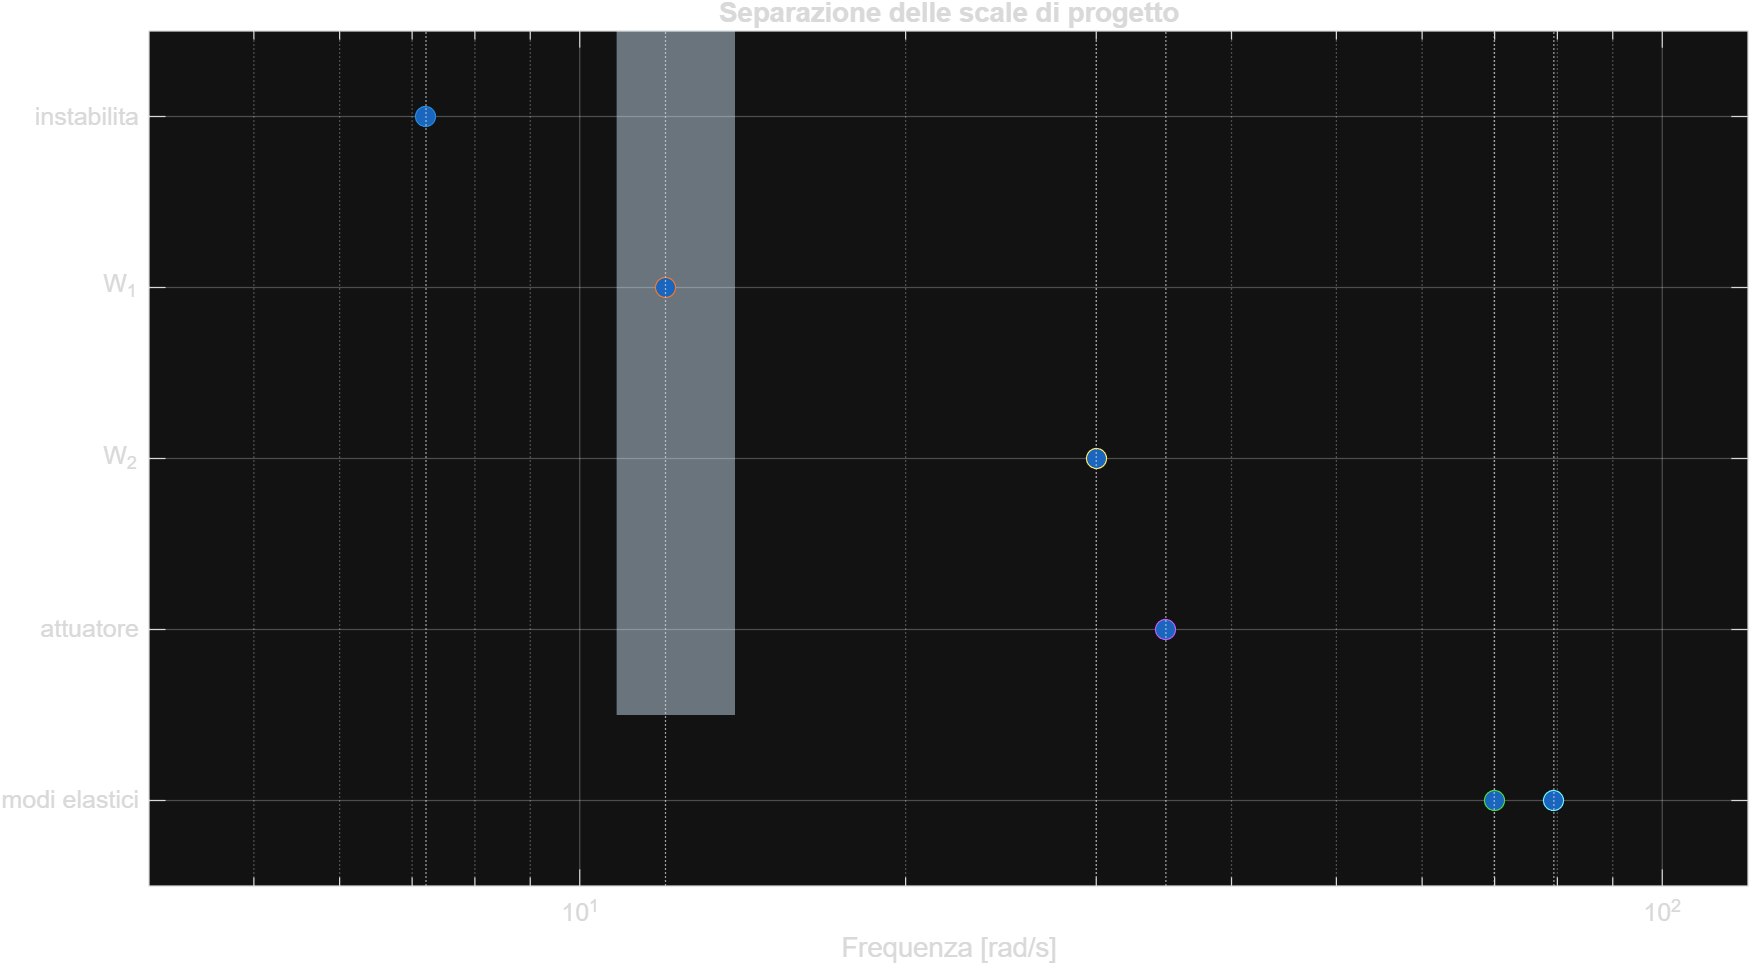
\includegraphics[width=0.79\textwidth]{figures/m5_spec_frequency_map.png}
\caption{Scale dinamiche utilizzate per motivare $\omega_B$ e $\omega_U$.}\label{fig:m5-map}
\end{figure}
